\documentclass{llncs}
%%%%%%%%%%%%%%%%%%%%%%%%%%%%%%%%%%%%%%%%%%%%%%%%%%%%%%%%%%%
%% package sillabazione italiana e uso lettere accentate
\usepackage[english]{babel}
\usepackage[T1]{fontenc}
\usepackage[utf8]{inputenc}
%%%%%%%%%%%%%%%%%%%%%%%%%%%%%%%%%%%%%%%%%%%%%%%%%%%%%%%%%%%%%

\usepackage{url}
\usepackage{xspace}
\usepackage{listings}
\usepackage{xcolor}
\usepackage{textcomp}

\makeatletter
%%%%%%%%%%%%%%%%%%%%%%%%%%%%%% User specified LaTeX commands.
\usepackage{manifest}

\makeatother


%%%%%%%
 \newif\ifpdf
 \ifx\pdfoutput\undefined
 \pdffalse % we are not running PDFLaTeX
 \else
 \pdfoutput=1 % we are running PDFLaTeX
 \pdftrue
 \fi
%%%%%%%
 \ifpdf
 \usepackage[pdftex]{graphicx}
 \else
 \usepackage{graphicx}
\usepackage{caption}
\usepackage{listings}
 \fi
%%%%%%%%%%%%%%%
 \ifpdf
 \DeclareGraphicsExtensions{.pdf, .jpg, .tif}
 \else
 \DeclareGraphicsExtensions{.eps, .jpg}
 \fi
%%%%%%%%%%%%%%%

\newcommand{\java}{\textsf{Java}}
\newcommand{\contact}{\emph{Contact}}
\newcommand{\corecl}{\texttt{corecl}}
\newcommand{\medcl}{\texttt{medcl}}
\newcommand{\msgcl}{\texttt{msgcl}}
\newcommand{\android}{\texttt{Android}}
\newcommand{\dsl}{\texttt{DSL}}
\newcommand{\jazz}{\texttt{Jazz}}
\newcommand{\rtc}{\texttt{RTC}}
\newcommand{\ide}{\texttt{Contact-ide}}
\newcommand{\xtext}{\texttt{XText}}
\newcommand{\xpand}{\texttt{Xpand}}
\newcommand{\xtend}{\texttt{Xtend}}
\newcommand{\pojo}{\texttt{POJO}}
\newcommand{\junit}{\texttt{JUnit}}

\newcommand{\action}[1]{\texttt{#1}\xspace}
\newcommand{\code}[1]{{\small{\texttt{#1}}}\xspace}
\newcommand{\codescript}[1]{{\scriptsize{\texttt{#1}}}\xspace}

% Cross-referencing
\newcommand{\labelsec}[1]{\label{sec:#1}}
\newcommand{\xs}[1]{\sectionname~\ref{sec:#1}}
\newcommand{\xsp}[1]{\sectionname~\ref{sec:#1} \onpagename~\pageref{sec:#1}}
\newcommand{\labelssec}[1]{\label{ssec:#1}}
\newcommand{\xss}[1]{\subsectionname~\ref{ssec:#1}}
\newcommand{\xssp}[1]{\subsectionname~\ref{ssec:#1} \onpagename~\pageref{ssec:#1}}
\newcommand{\labelsssec}[1]{\label{sssec:#1}}
\newcommand{\xsss}[1]{\subsectionname~\ref{sssec:#1}}
\newcommand{\xsssp}[1]{\subsectionname~\ref{sssec:#1} \onpagename~\pageref{sssec:#1}}
\newcommand{\labelfig}[1]{\label{fig:#1}}
\newcommand{\xf}[1]{\figurename~\ref{fig:#1}}
\newcommand{\xfp}[1]{\figurename~\ref{fig:#1} \onpagename~\pageref{fig:#1}}
\newcommand{\labeltab}[1]{\label{tab:#1}}
\newcommand{\xt}[1]{\tablename~\ref{tab:#1}}
\newcommand{\xtp}[1]{\tablename~\ref{tab:#1} \onpagename~\pageref{tab:#1}}
% Category Names
\newcommand{\sectionname}{Section}
\newcommand{\subsectionname}{Subsection}
\newcommand{\sectionsname}{Sections}
\newcommand{\subsectionsname}{Subsections}
\newcommand{\secname}{\sectionname}
\newcommand{\ssecname}{\subsectionname}
\newcommand{\secsname}{\sectionsname}
\newcommand{\ssecsname}{\subsectionsname}
\newcommand{\onpagename}{on page}

\newcommand{\xauthA}{Alessio Tonioni}
\newcommand{\xauthB}{NameB StudentB}
\newcommand{\xauthC}{NameC StudentC}
\newcommand{\xfaculty}{Faculty of Engineering}
\newcommand{\xunibo}{Alma Mater Studiorum -- University of Bologna}
\newcommand{\xaddrBO}{viale Risorgimento 2}
\newcommand{\xaddrCE}{via Venezia 52}
\newcommand{\xcityBO}{40136 Bologna, Italy}
\newcommand{\xcityCE}{47023 Cesena, Italy}

%
% Comments
%
%%% \newcommand{\todo}[1]{\bf{TODO:}\emph{#1}}


%-----------------------------Codice disegno--------------------------
\lstset{ %
  backgroundcolor=\color{white},   % choose the background color; you must add \usepackage{color} or \usepackage{xcolor}
  basicstyle=\footnotesize,        % the size of the fonts that are used for the code
  breakatwhitespace=false,         % sets if automatic breaks should only happen at whitespace
  breaklines=true,                 % sets automatic line breaking
  captionpos=b,                    % sets the caption-position to bottom
  commentstyle=\color{green},      % comment style
  deletekeywords={...},            % if you want to delete keywords from the given language
  escapeinside={\%*}{*)},          % if you want to add LaTeX within your code
  extendedchars=true,              % lets you use non-ASCII characters; for 8-bits encodings only, does not work with UTF-8
  frame=single,                    % adds a frame around the code
  keepspaces=true,                 % keeps spaces in text, useful for keeping indentation of code (possibly needs columns=flexible)
  keywordstyle=\color{blue},       % keyword style
  morekeywords={*,...},            % if you want to add more keywords to the set
  numbers=left,                    % where to put the line-numbers; possible values are (none, left, right)
  numbersep=5pt,                   % how far the line-numbers are from the code
  numberstyle=\tiny\color{gray},   % the style that is used for the line-numbers
  rulecolor=\color{black},         % if not set, the frame-color may be changed on line-breaks within not-black text (e.g. comments (green here))
  showspaces=false,                % show spaces everywhere adding particular underscores; it overrides 'showstringspaces'
  showstringspaces=false,          % underline spaces within strings only
  showtabs=false,                  % show tabs within strings adding particular underscores
  stepnumber=1,                    % the step between two line-numbers. If it's 1, each line will be numbered
  stringstyle=\color{red},         % string literal style
  tabsize=2,                       % sets default tabsize to 2 spaces
  title=\lstname                   % show the filename of files included with \lstinputlisting; also try caption instead of title
}

\begin{document}

\title{Attività progettuale di ingegneria dei sistemi software\\
 progetto "Line follower"}

%%% \author{\xauthA \and \xauthB}
\author{\xauthA}

\institute{%
%%%  \xunibo\\\xaddrCE, \xcityCE\\\email{\{nameA.studentA, nameB.studentB\}@studio.unibo.it}
  \xunibo\\\xaddrBO, \xcityBO\\\email\ alessio.tonioni@studio.unibo.it
}

\maketitle

%% \begin{abstract}
%% \footnotesize
%%This a Latex template to be used for the reports of Software Engineering.
%%\keywords{Software engineering, managed software development, reports, ....}
%%\end{abstract}

%%% \sloppy

%===========================================================================
\section{Introduction}
\labelsec{intro}
The aim of this project it's to realize an independent controller that controls a robot and makes it capable of following a line on the ground.
Furthermore the focus of the work is on the property of the software developed and how to organize the work with the purpose of obtaining a piece of reliable and reusable code. \\
%===========================================================================

%===========================================================================
\section{Vision}
\labelsec{Vision}
The development of the controller should be fully automatable given the fundamental parameters of the robot, so the controller should be as general purpose as possible and should not be bonded to a specific type of robot or to a sensors configuration. After the initial development new controllers should not be implemented by code, but automatically with the help of simplified language capable of describe exhaustively the robot.
%===========================================================================

%===========================================================================
\section{Goals}
\labelsec{Goals}
Realize an independent controller to make a robot able to follow a line on the ground.\\ 
%===========================================================================

%===========================================================================
\section{Requirements}
\labelsec{Requirements}
Realize an independent controller to make a robot able to follow a line on the ground perceptible with on-board sensors.\\
Normally the robot it's remote-controlled from a remote device, but when requested the line's follower takes the control of the robot and drives it till new command are given. \\
At any given moment during the execution of the controller new commands could be sent from the remote device, when this happen the controller stop working and the robot must returns to remote-controlled only.
%===========================================================================

 
%===========================================================================
\section{Requirement analysis}
\labelsec{ReqAnalysis}

%===========================================================================
\subsection{Use cases}
\labelssec{UseCases}
\begin{center}
  \makebox[\textwidth]{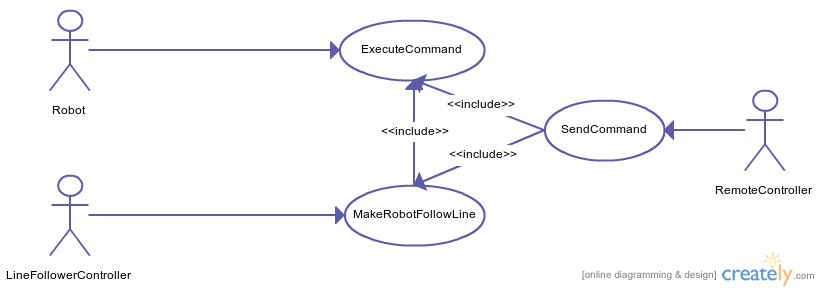
\includegraphics[width=\textwidth]{img/PIDUseCases.png}}
\end{center}

%===========================================================================
\subsection{Scenarios}
\labelssec{Scenarios}
\textbf{ExecuteCommand:}\\
Actor: robot\\
Post-condition: the robot is executing a command.\\
\\
Main scenario:
\begin{itemize}
	\item The robot is asked to execute a simple command
	\item The robot starts to execute the command and continues till a new one is executed
\end{itemize}
 
\noindent{\textbf{MakeRobotFollowLine:}}\\
Actor: Line follower controller\\
Post-condition: the robot is moving autonomously and it's following a line on the floor\\
Main scenario:
\begin{itemize}
	\item The robot is asked to start following a line
	\item The robot starts to follow the line and continues till a new command are requested
\end{itemize}

\noindent{\textbf{ReceiveCommand:}}\\
Actor: remote controller\\
Pre-condition: the remote controller knows how to communicate with the robot\\
Post-condition: the robot executes the command sent.\\
Main scenario:
\begin{itemize}
	\item A command or the request to start a line follower controller is sent from the remote controller.
	\item The robot starts to execute what is requested to do.
\end{itemize}
 



%============================================================================
\subsection{Glossary}
\begin{center}
	\begin{tabular}{| p{0.3\textwidth} | p{0.7\textwidth}|}
		\hline
 		\textbf{Term }         &  \textbf{Meaning}   \\
		\hline
		Command &Basic action that the robot it's capable of interpret and execute. \\
		\hline
		Independent Controller &Autonomous entity capable of control a robot giving it command. \\
		\hline 
		Line  &Mark perceptible with on-board sensors. \\
		\hline
		Remote device  &Entity independent from the robot able to communicate with it. It can ask to a certain robot the execution of a command or the start of a line follower controller. \\
		\hline
		Robot   &Entity capable of interpret command. \\
		\hline
	\end{tabular}
\end{center}

%===========================================================================

\subsection{(Domain)model}
The domain it's made of at least two physically separated macro entity:\\

\noindent{\textbf{Remote-device:}}\\
Entity capable of connect in some way to the robot and send it command, it could be formalized with this interface.
\lstinputlisting[language=Java,basicstyle=\small\ttfamily,breaklines=true,showtabs=false,showspaces=false,breakatwhitespace=true]{/home/alessio/git/AttivitaProgettuale/ModelInterfaces/src/interfaces/RemoteDevice.java}

\noindent{\textbf{Robot:}}\\
The physical entity robot could be decomposed in three sub-system:
\begin{itemize}
	\item \textbf{Executor:} interpret of commands already realized, it could be formalized with the given interface:
		\lstinputlisting[language=Java,basicstyle=\small\ttfamily,breaklines=true,showtabs=false,showspaces=false,breakatwhitespace=true]{/home/alessio/git/AttivitaProgettuale/it.unibo.iot.robot/src/it/unibo/iot/robot/IRobot.java}
	\item \textbf{Command Receiver:} entity with the task of receiving messages from the remote devices, interpret it and translate them in command for the robot or the line follower. It could be formalized with this interface.
		\lstinputlisting[language=Java,basicstyle=\small\ttfamily,breaklines=true,showtabs=false,showspaces=false,breakatwhitespace=true]{/home/alessio/git/AttivitaProgettuale/ModelInterfaces/src/interfaces/ICommandReceiver.java}
	\item \textbf{Line follower:} entity that when started takes control of a robot with the purpose of making it follow a line on the ground, it must be stopped when requested from the outside and should be able to communicate with the sensors on the robot. If possible this component should be reusable across different robots or sensors configuration. It could be formalized with this interface:
		\lstinputlisting[language=Java,basicstyle=\small\ttfamily,breaklines=true,showtabs=false,showspaces=false,breakatwhitespace=true]{/home/alessio/git/AttivitaProgettuale/ModelInterfaces/src/interfaces/ILineFollower.java}
\end{itemize}
This three entities could be active at the same time: the "Command Receiver", for example, is always listening for incoming messages meanwhile the robot is executing a command or the controller is following a line. The three sub-systems are all inside the robot system because "executor" and "line follower" must communicate with external device on board on the robot: engine and sensors respectively; Command receiver instead must communicate with executor.

%==========================================================================
\subsection{Test plan}
In order to introduce automatic test cases a modified robot must be modelled:
\lstinputlisting[language=Java,basicstyle=\small\ttfamily,breaklines=true,showtabs=false,showspaces=false,breakatwhitespace=true]{/home/alessio/git/AttivitaProgettuale/ModelInterfaces/src/test/MyIRobot.java}
Now the interface of the model can be tested:
\lstinputlisting[language=Java,basicstyle=\small\ttfamily,breaklines=true,showtabs=false,showspaces=false,breakatwhitespace=true]{/home/alessio/git/AttivitaProgettuale/ModelInterfaces/src/test/LineFollowerTest.java}
\lstinputlisting[language=Java,basicstyle=\small\ttfamily,breaklines=true,showtabs=false,showspaces=false,breakatwhitespace=true]{/home/alessio/git/AttivitaProgettuale/ModelInterfaces/src/test/RemoteDeviceTest.java}
%===========================================================================
\section{Problem analysis}
\labelsec{ProblemAnalysis}

%===========================================================================
\subsection{Logic architecture}
The software system is composed of at least two physically separated entities that must communicate, the semantic of the communication its asynchronous and mono directional. A typical message exchange of the whole system could be pictured with this schema:
\begin{center}
  \makebox[\textwidth]{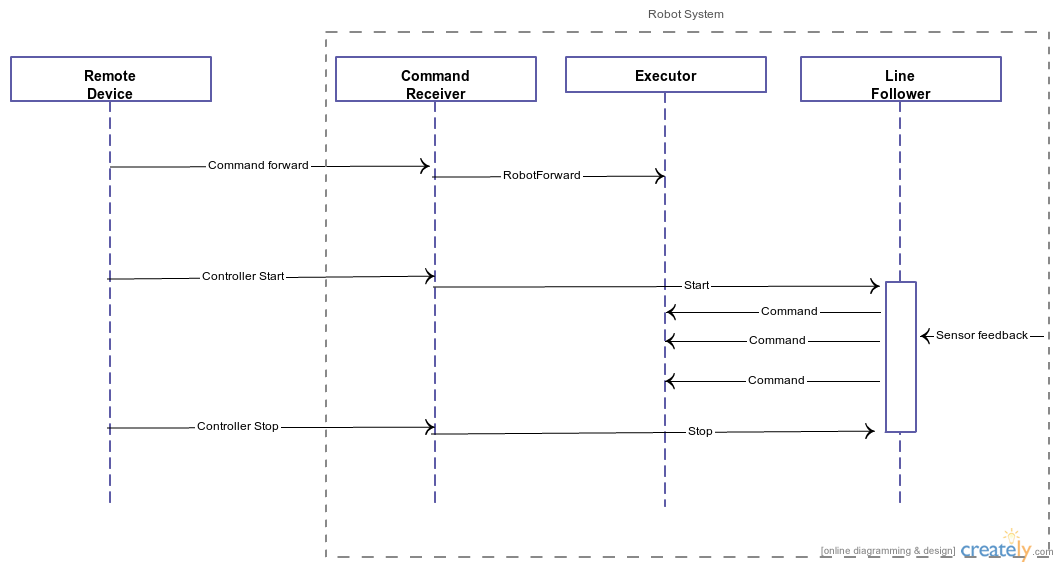
\includegraphics[width=\textwidth]{img/SequenceDiagram.png}}
\end{center}
All the messages are asynchronous, the content of the message between "Remote device" and "Command receiver" should conform to a certain grammar in order to make the communication possible.\\
The messages directed to the "executor" should conform to the given IRobot interface, for example each message could correspond to a proper call of the "execute()" method of the IRobot.\\
The messages of start and stop from the "command receiver" to the "line follower" could be seen as creation and destruction of the "line follower", furthermore this follower must be able to receive incoming messages from the sensors so it must communicate with them.\\
As seen all the interaction between the remote device and the robot system are transmitted through the "command receiver" that it's the only point of communication between the robot system and the outside world, the communication is mono directional, so there are no feedbacks from the robot on the correct execution of the requested action.\\
The sensors' feedbacks are produced independently from the rest of the system, this type of messages are asynchronous and are already implemented using an observer pattern to be notified when new measurement are available.\\

From this representation we can see that the "executor" is a completely passive entity capable only of execute commands when requested, instead the "line follower" is an active entity with a limited life span that could be created and destroyed at any given time, at this level of abstraction we are not interested on how the controller does it's job, the only thing it must guarantee is that when activated the robot start to follow the line. The "Command receiver" is an interpret that translate the request of the remote device in command for the "executor" and the "line follower", it must be created at the startup of the system and must remain active till the system is turned off.\\
Every "command receiver" must have an unique identifier so that a remote device can only send message to a specific one. In this architecture is possible that more than one remote devices send messages to the same command receiver, in this case there's no priority and the execution of the messages is FIFO. 

\subsection{Abstraction gap}
The infrastructure to control the robot engines and sensors is already developed, so there should be no problem for the interaction with physical devices. The communication between the entities could be implemented using standard tcp/ip protocol in order to be cross platform and scalable. The main abstraction gap is the absence of a way to tune the line follower controller for a certain robot in a fully automated way. Some experimental approach using genetic computation will be presented later, but the result are still not perfect.    

\newpage
%===========================================================================
\section{Project}
\labelsec{Project}
%===========================================================================

\subsection{Structure}
The overall structure of the system conform to the one presented in the logic architecture part, however there's some little clarification on how the single entities are implemented.\\

\noindent{\textbf{Command Receiver --> listenerController:} project it.unibo.RobotServer}\\
To achieve the maximum independence from the technology used in different systems, the command receiver is realized as a simple tcp server, and the messages are so composed:
\begin{itemize}
	\item 1 byte for the size of the message
	\item A string encoded using UTF-8 standard
\end{itemize} 
In order to be correctly interpreted the string must follow this grammar:
\lstset{language=Java}
\begin{lstlisting}
SCOPE: MSGTYPE
MSGTYPE: COMMANDMSG | CONTROLLERMSG
COMMANDMSG: "cmd " COMMANDTYPE SPEED
CONTROLLERMSG: "cnt " CNTTYPE SPEED FORWARD
COMMANDTYPE: "forward" | "backward" | "left" | "right" | "fordwardRight" | "forwardLeft" | "backwardRight" | "backwardLeft" | "stop"
CNTTYPE: "PID" | "StateBiLine" | "StateMonoLine" | "PIDFinale"
SPEED: integer between [0,100]
FORWARD: "true"|"false"
\end{lstlisting}
The "command receiver" uses an external component, implementation of \textbf{ICommandExecutor}, to make the physical robot execute commands or to start the "line follower" controller, in this way some parts of the server are reusable for different physical robot.\\

\noindent{\textbf{Remote Device:} project RemoteControlRobot\\}
For testing purpose the remote device is implemented as a simple Windows phone app, the only thing it must do is to connect to the tcp server on the robot and send to it message composed as described above.\\

\noindent{\textbf{LineFollower --> ILineFollower} project it.unibo.lineFollower}\\
This component must be able to control autonomously the robot but at the same time must be stoppable, for this reason the ILineFollower interface extends Runnable so every controller can be instantiated as a thread that iteratively calculates the corrective commands to make the robot follow a line till someone kills it using the method terminate().\\
The core of the project is the implementation of the ILineFollower interface, after some tests with different solutions the final implementation uses a PID controller to calculate the correction, an external \textbf{IErrorUpdater} to keep track of the current tracking error of the robot using a specific sensors configuration and an external \textbf{ICommandExecutor} to make the robot able to physically execute the corrective commands.  \\
\begin{center}
  \makebox[\textwidth]{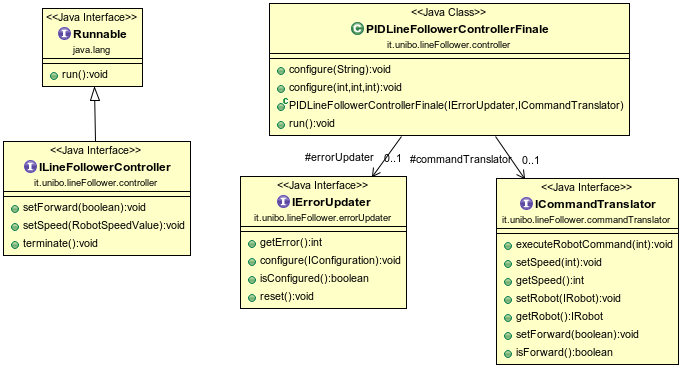
\includegraphics[width=\textwidth]{img/LineFollower.png}}
\end{center}

\noindent The error calculated from an implementation of \textbf{IErrorUpdater} must be an integer between [-100,100] where 0 means no error, -100 totally wrong on the left and +100 totally wrong on the right. Through this measure of the error the \textbf{PID} controller generates another integer which represents the correction that must be applied to the robot to make it return on the correct track, is now the turn of the \textbf{ICommandExecutor} to take this integer and translate it in command that the robot is capable of execute.\\
The behavior of the PID controller depends not only on the IErrorUpdater that generates the error, but also on 3 constants (Proportional-Integral-Derivative) that are sets with the two configure() method, good constants can make the controller more reactive and less prone to error.\\
Every constant has a specific role:
\begin{itemize}
	\item \textbf{Proportional: } higher values make the controller react more strongly to errors.
	\item \textbf{Integral: } higher values make the controller react  more strongly when errors are presents from long time.
	\item \textbf{Derivative: } higher values make the controller react faster when the errors happen.
\end{itemize}

\noindent Using this structure the controller can be reused with any sets of sensors or robot and to perform several different tasks, for example it could be used to run a robot inside an aisle just creating different implementation of the IErrorUpdater.\\

\subsection{Interaction}
The communication between the remote device and the command executor is realized using standard tcp socket. Tcp is preferred over udp because ensure the correct order of arrival of the commands.\\
All the interaction inside the robot entities instead are implemented as simple procedure call. \\
A typical interaction of the system can be pictured like this:
\begin{center}
  \makebox[\textwidth]{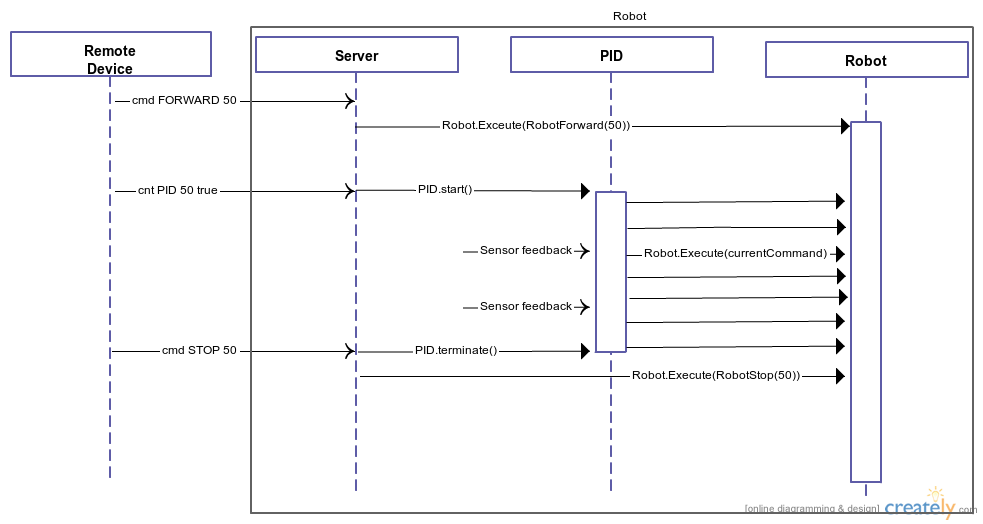
\includegraphics[width=\textwidth]{img/InteractionDiagram.png}}
\end{center}


\subsection{Behavior}
The overall behavior of the pid controller follow this state machine 
\begin{center}
  \makebox[\textwidth]{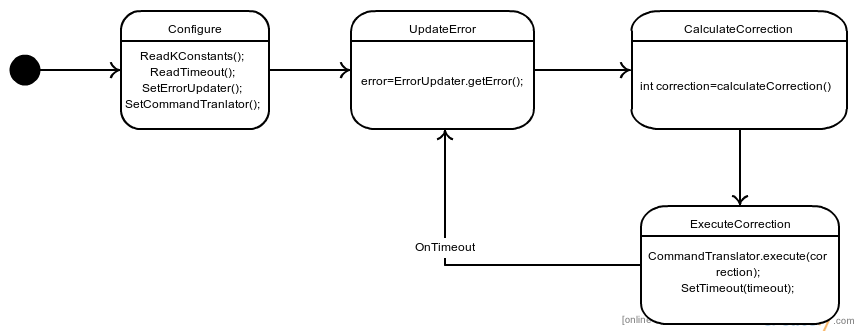
\includegraphics[width=\textwidth]{img/PIDFinaleStateMachine.png}}
\end{center}

%===========================================================================
\newpage
\section{Implementation}
\labelsec{Implementation}
Given the overall structure the implementation is quite simple and does not presents difficult point.  
As said above the structure is very reusable because of the modularity and adaptability, but it must be properly \textbf{tuned} before starting. Tuning corresponds to properly sets the 3 constants of the PID controller in order to make it able to control a specific robot.\\

\noindent Before using a controller there must always be a phase of long testing to find the proper constant for the robot and the sensors' configuration. In order to try to automatize this task is been tested a method based on Evolutionary computation: using a simulator and a lot of iterations we try to find the best possible constants to control that particular simulated robot. The more the simulated robot behavior is close to the real one the more this technique can be useful. \\

\begin{center}
  \makebox[\textwidth]{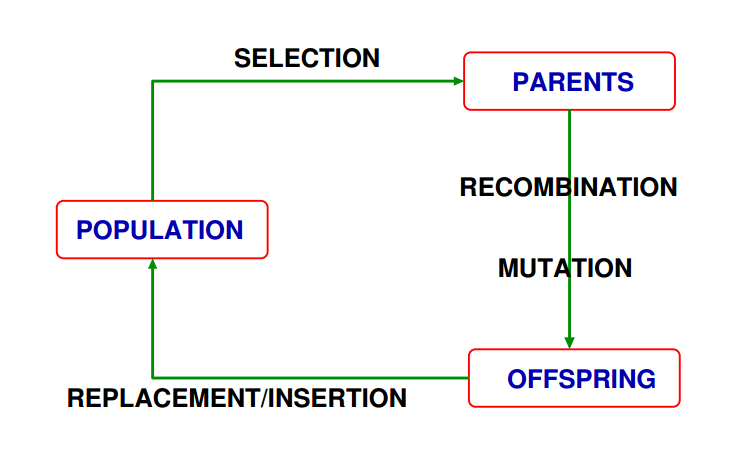
\includegraphics[width=\textwidth]{img/evoluzione.png}}
\end{center}

\noindent The genetic computation program starts from a population of individuals, in our case different combination of PID constants, and at each iteration gives at all of them a score, called fitness, based on how well they behave. From this population a new one is generated recombining the best current solutions and adding some random mutation, the new generation created should perform better than the one before and the iteration could restarts. After a certain number of iteration we should obtain a good individual among the population, so a good set of constants.\\
In order to implement this algorithm in the most general way possible the logic of population creation and score calculation are relegated to two external components: \textbf{IGenerator} and \textbf{IFitnessCalculator}. For example the implementation of IFitnessCalculator for the PID controller uses a simulator to get the score of each individual.
\begin{center}
  \makebox[\textwidth]{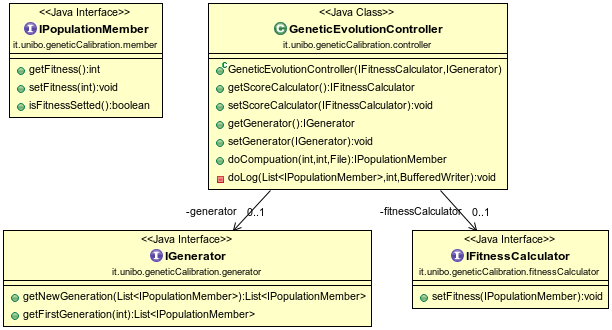
\includegraphics[width=\textwidth]{img/geneticCalibration.png}}
\end{center} 


%===========================================================================

%===========================================================================
\section{Testing}
\labelsec{testing}
All the system was tested using a differential drive robot with two line sensors and a windows phone for the remote device. The results are quite good, but the constants calculated using the genetic computation needs a refinement by hand probably because of the too simplistic simulation.
%===========================================================================

%===========================================================================
\section{Deployment}
\labelsec{Deployment}
The system is deployed as a single .jar for the robot and an application for the remote device. In order to work properly the jar needs also a series of configuration file both for how to interact with sensors and motors and for how to configure the controller.
%===========================================================================

%===========================================================================
\section{Maintenance}
\labelsec{Maintenance}
%===========================================================================
\newpage

%===========================================================================
\section{Information about the author}
\labelsec{Author}
%===========================================================================

\vskip.5cm
%%% \begin{figure}
\begin{tabular}{ | c |  }
\hline
  % after \\: \hline or \cline{col1-col2} \cline{col3-col4} ...
  Photo of the author 
  \\
\hline
   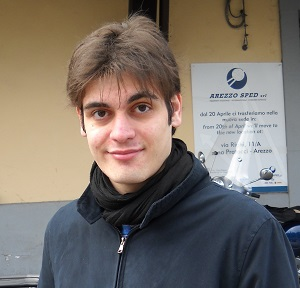
\includegraphics[scale = 0.45]{img/foto_autore.jpg}
  \\
\hline
\end{tabular}


%%% \begin{itemize}
%%% \item Titolo di studio:\\ \\
%%% \item Interessi particolari:\\ \\
%%% \item Ha sostenuto fino ad oggi il seguente numero di esami:\\ \\
%%% \item Deve ancora sostenere i seguenti esami del I anno:\\ \\
%%% \item Prevede di svolgere un tirocinio presso:\\ \\
%%% \item Prevede di laurearsi nella sessione:\\ \\
%%% \item Intende proseguire gli studi per conseguire: \\  \\  \\
%%%   	presso la sede universitaria di: \\ \\
%%% \item Intende entrare subito nel mondo del lavoro presso : \\ \\
%%% \end{itemize}

 
\appendix


\bibliographystyle{abbrv}
\bibliography{biblio}

\end{document}














